\documentclass[landscape]{foils} 
\newif\ifpdf
\ifx\pdfoutput\undefined
\pdffalse % we are not running PDFLaTeX
\else
\pdfoutput=1 % we are running PDFLaTeX
\pdftrue
\fi

\ifpdf
\usepackage[pdftex]{graphicx}
\else
\usepackage{graphicx}
\fi

\ifpdf
\DeclareGraphicsExtensions{.pdf, .jpg, .tif, .png}
\else
\DeclareGraphicsExtensions{.eps, .jpg}
\fi

%\usepackage{pslatex}
\usepackage{tabularx,dcolumn, graphicx, amsfonts,amsmath}  
\usepackage[sectionbib]{natbib}
\bibliographystyle{apalike}
\usepackage{picinpar}
\usepackage{multirow}
\usepackage{rotating}
\usepackage{paralist} %compactenum
\setlength{\voffset}{-0.5in}
%\setlength{\hoffset}{-0.5in}
%\setlength{\textwidth}{10.5in}
\setlength{\textheight}{7in}
\setlength{\parindent}{0pt}
%\pagestyle{empty}
%\renewcommand{\baselinestretch}{2.0}
\DeclareMathSymbol{\expect}{\mathalpha}{AMSb}{'105}
\def\p{\rm p}
\def\pp{\rm P}
% this are commands that come with the color package
\usepackage{color}
\usepackage{fancyhdr}


\pagestyle{empty}
%define colors
\definecolor{mediumblue}{rgb}{0.0509,0.35,0.568}
\definecolor{blue}{rgb}{0.0109,0.15,0.468}
\definecolor{black}{rgb}{0.04,0.06,0.2}
\definecolor{darkblue}{rgb}{0.03,0.1,0.2}
\definecolor{darkgreen}{rgb}{0.03,0.5,0.2}
\definecolor{lightblue}{rgb}{0.85,0.9333,0.95}
\definecolor{lightblue2}{rgb}{0.270588, 0.45098, 0.701961}
\definecolor{white}{rgb}{1.0,1.0,1.0}
\definecolor{yellow}{rgb}{0.961,0.972,0.047}
\definecolor{red}{rgb}{0.9,0.1,0.1}
\definecolor{orange}{rgb}{1.0,0.4,0.0}
\definecolor{grey}{rgb}{0.5,0.5,0.5}
\definecolor{violet}{rgb}{0.619608, 0.286275, 0.631373}
\definecolor{mybackgroundcolor}{rgb}{1.0,1.0,1.0}

%\definecolor{light}{rgb}{.5,0.5,0.0}
\definecolor{light}{rgb}{.3,0.3,0.3}

% sets backgroundcolor for whole document 
\pagecolor{mybackgroundcolor}
% sets text color
%\color{black}
% see below for an example how to change just a few words
% using \textcolor{color}{text}

\font \courier=pcrb scaled 2000
\newcommand{\notetoself}[1]{{\textsf{\textsc{\color{red} #1}}}\\}

\newcommand{\answer}[1]{{\sf \color{red} #1}}

\usepackage{pdfpages}

\newcommand{\section}{\secdef \newsection\newsection}
%\renewcommand{\labelitemi}{\includegraphics[width=5mm]{images/bullet.pdf}}
\newcommand{\newsection}[1]{%
{
	\par\flushleft\large\sf\bfseries \vskip -2cm #1\\\rule[0.7\baselineskip]{\textwidth}{0.5mm}\par}}

\newcommand{\subsection}{\secdef \test\test}
\newcommand{\test}[1]{%
	{\par\flushleft\normalsize\sf\bfseries #1: }}
\newcommand{\M}{\mathcal{M}}
\newcommand{\prob}{{\rm Prob~}}
\def\showy#1{{\normalsize\sf\bfseries #1}}
\def\donotuse#1{}

\newcommand{\entrylabel}[1]{\mbox{#1}\hfil}
\newenvironment{entry}
	{\begin{list}{}%
		{\renewcommand{\makelabel}{\entrylabel}%
		\setlength{\labelwidth}{35pt}%
		\setlength{\leftmargin}{\labelwidth+\labelsep}%
	}%
	{\end{list}}}

\newcommand{\poltext}{{\copyright\ 2002--2010 by Paul O. Lewis -- Modified by  Mark Holder with permission from Paul Lewis}}

\newcommand{\pol}{{\footnotesize \poltext}}
\newcommand{\myBackground}{\begin{picture}(0,0)(0,0)  \put(-40,-70){\makebox(0,0)[l]{\includegraphics[width=33cm]{images/baby_blue.jpg}}} \end{picture}}
\newcommand{\myFooter}{}
%\begin{picture}(0,0)(0,0)
%	\put(0,-185){\pol}
%\end{picture}}
\newcommand{\myNewSlide}{\newpage\myFooter} % \myBackground}

\usepackage{url}
\usepackage{hyperref}
\hypersetup{backref,  linkcolor=blue, citecolor=black, colorlinks=true, hyperindex=true}

\usepackage{pdfpages}
\usepackage{bm}
\usepackage{ifsym}

\begin{document}

\myNewSlide
\huge 
Thanks to Paul Lewis, Joe Felsenstein, and Peter Beerli for slides.

\myNewSlide
\section*{Reasons phylogenetic inference might be wrong}
\Large
\begin{compactenum}
	\item Our data might be wrong (``garbage in garbage out'')
	\item {\em Systematic error} -- our inference method might not be sophisticated enough
	\item \underline{{\em Random error}} -- We might not have enough data, so we are misled by sampling error.
\end{compactenum}

(or it could be some combination of these).

\myNewSlide
\section*{Is our data set large enough to avoid random errors?}

This evening:
\begin{enumerate}
	\item Bootstrapping;
	\item Topology tests (KH, SH, AU, aLRT, aBayes, $\ldots$);
	\item Discussion of the theory underlying this plethora of testing methods, and the history of the debates around bootstrapping in phylogenetics;
	\item brief lab on how to use {\tt Seq-Gen} to conduct parametric bootstrapping.
\end{enumerate}


\myNewSlide
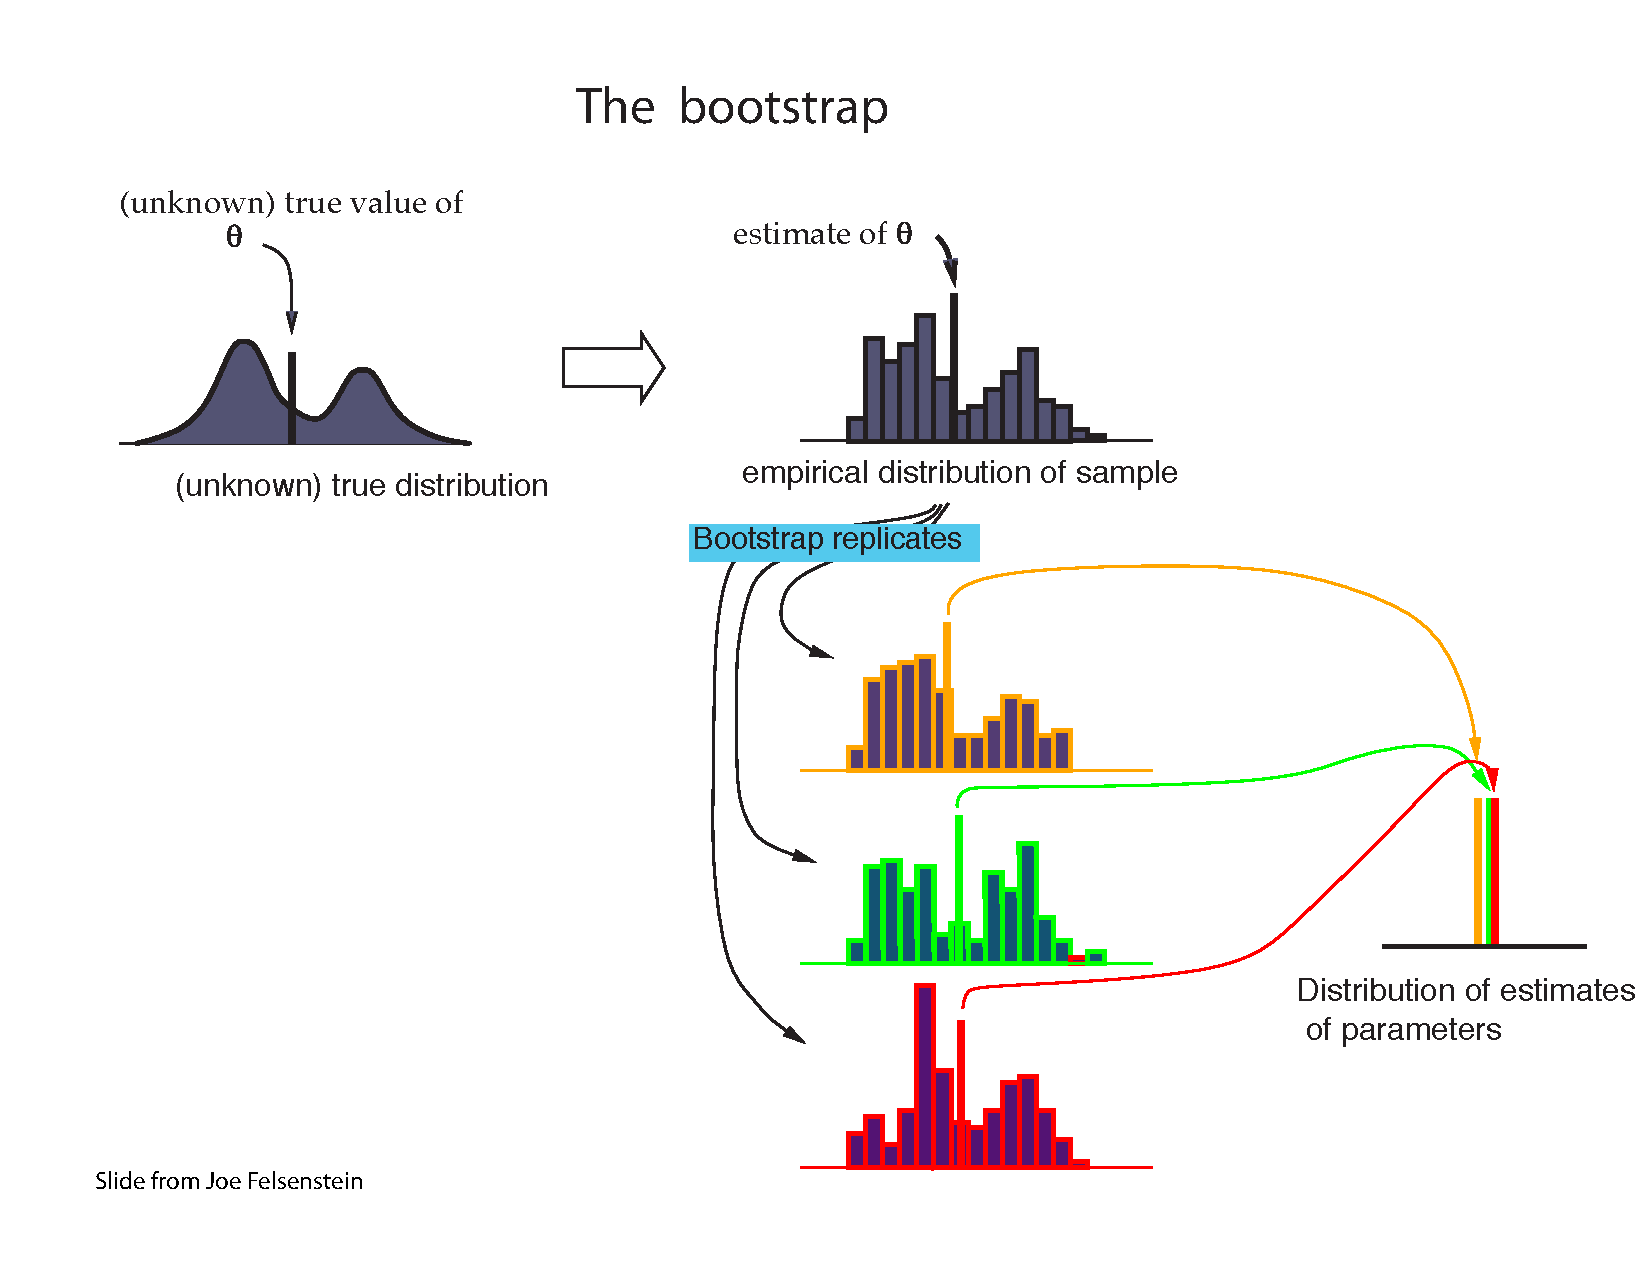
\includepdf[pages={1}]{../newimages/JoeFelsBootFig1.pdf} 

\myNewSlide
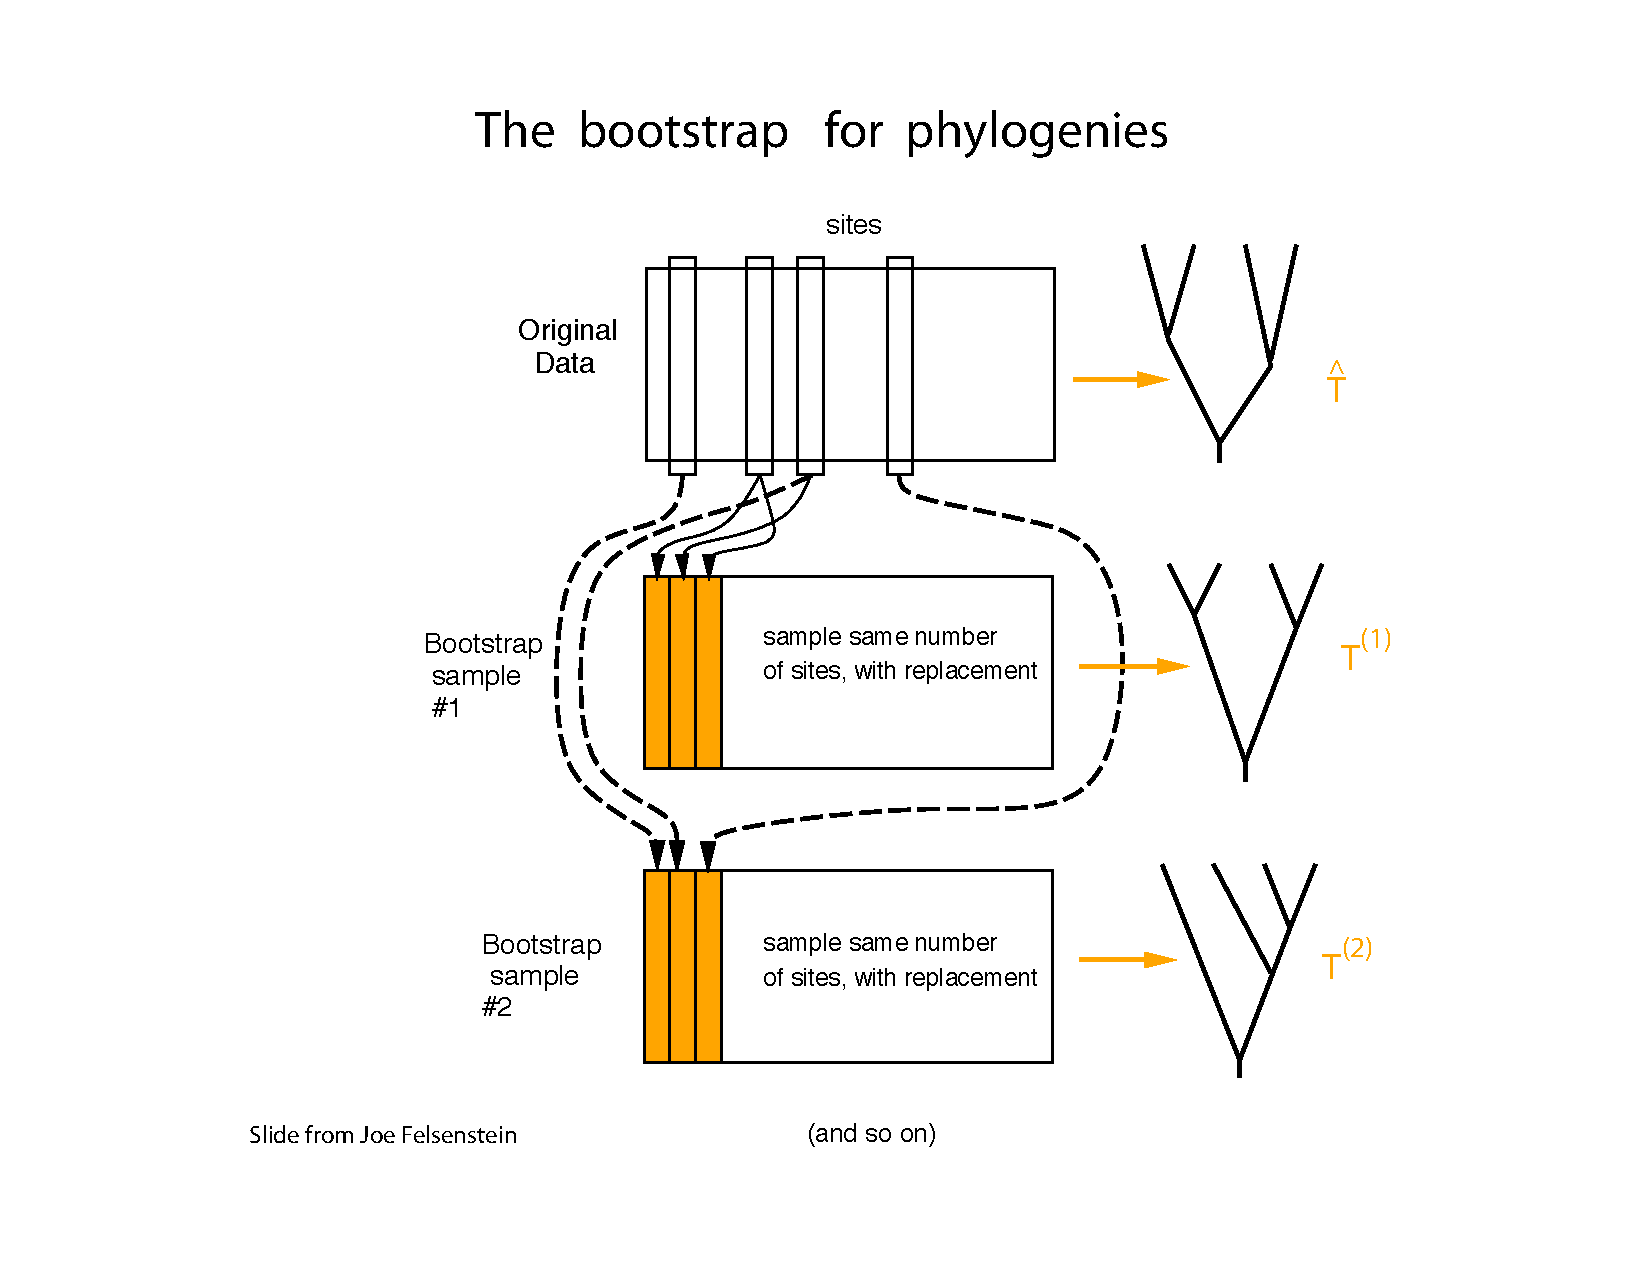
\includepdf[pages={1}]{../newimages/JoeFelsBootFig2.pdf} 

\myNewSlide
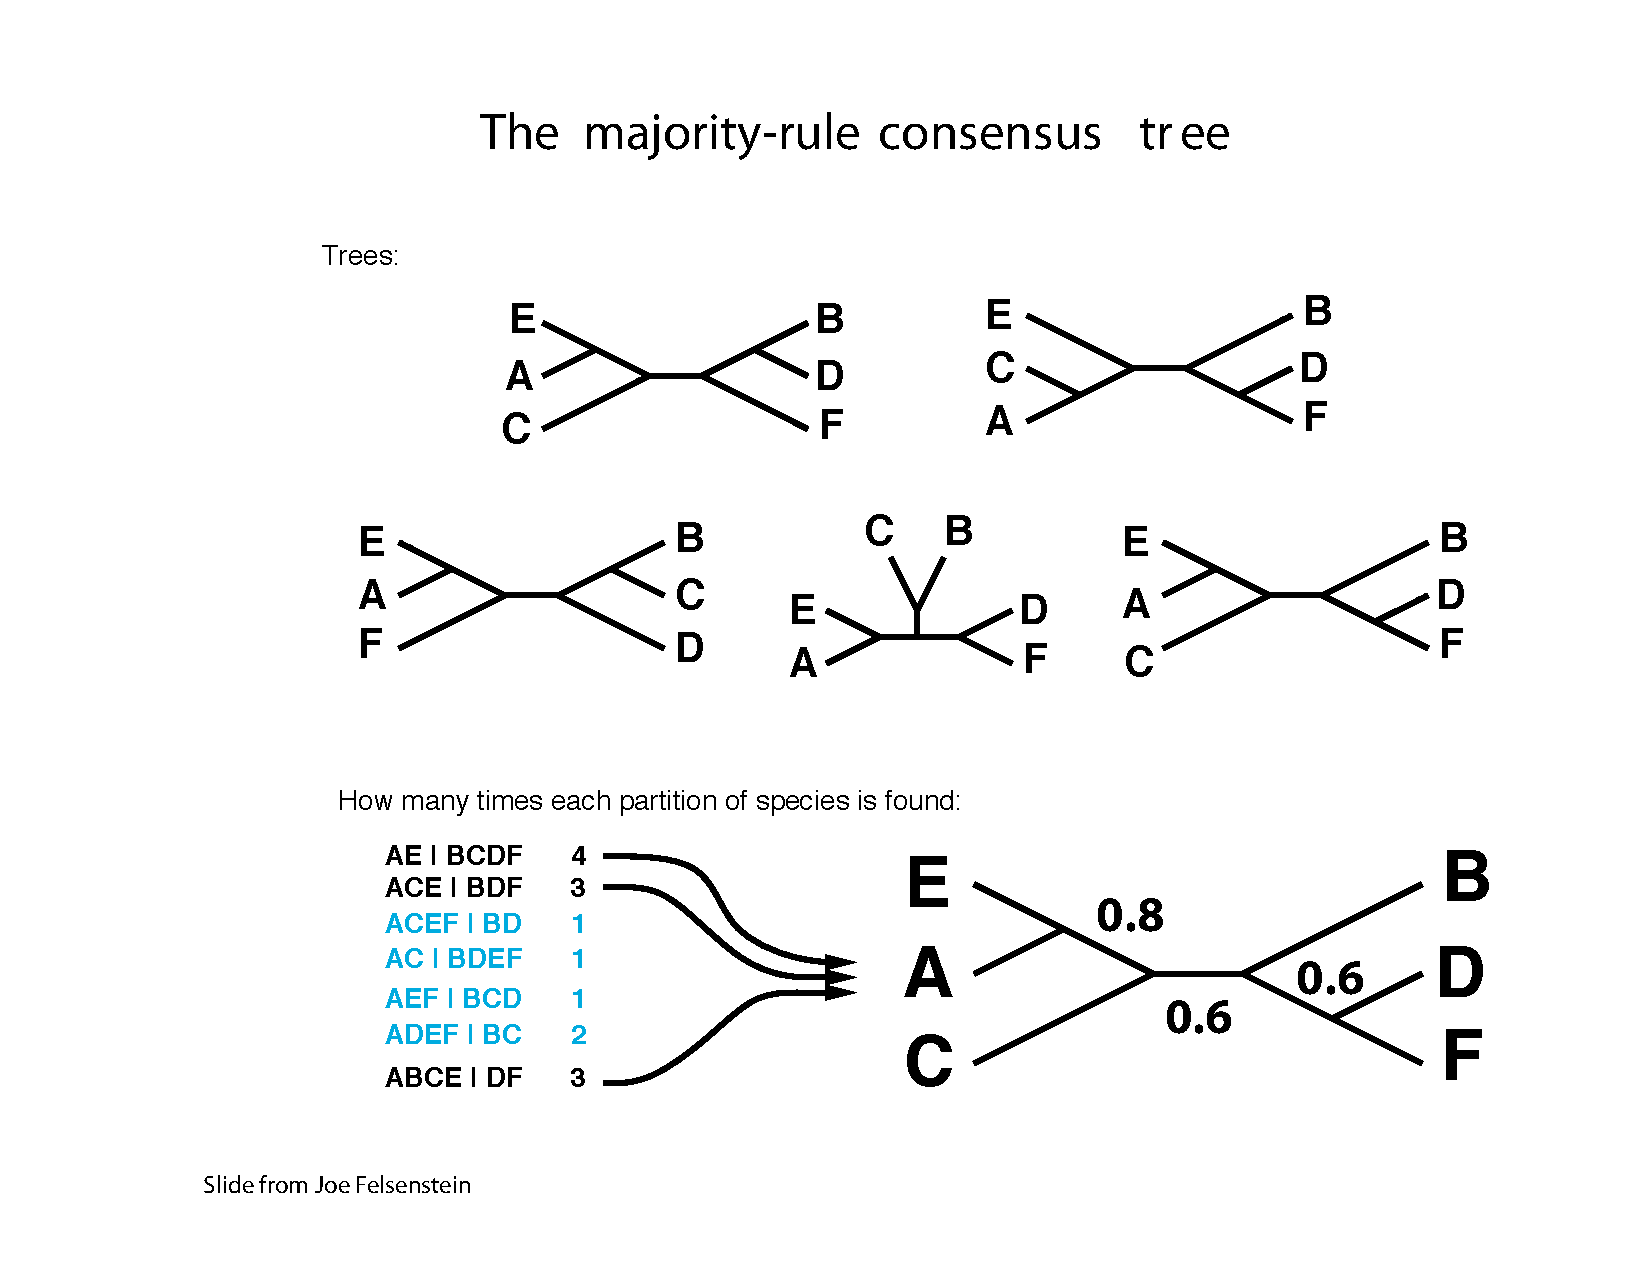
\includepdf[pages={1}]{../newimages/JoeFelsBootFig3.pdf} 



\end{document}

\myNewSlide
\section*{Frequentist phylogenetic hypothesis testing?}
If we have a tree, $T_0$, in mind {\em a priori}, then how can we answer the question:

``Based on this data, should we reject the tree?'' 

Clearly if $\hat{T}\neq T_0$, then there is a possiblity that we should reject $T$.  

But how do we calculate a p-value?

\myNewSlide
\section*{Frequentist phylogenetic hypothesis testing? (cont)}
What is our test-statistic? {\color{red} Difference in support between the null tree and the preferred tree.}

How do we find the null-distribution for the test statistic? {\color{red} Simulation}

\myNewSlide
\includepdf[pages={2}]{../lec14Testing/images/polBremer.pdf} 

\myNewSlide
\section*{Testing 2 trees}
\Large
Test statistic: The difference in score, $\delta$, between two trees chosen {\em a priori}.

Null hypothesis: Both trees are equally good explanations of the truth.

\[E(\delta) = 0\]

Is $\delta$ so large that we reject the null?\\ What if $\delta=-9$, should we reject the null?

\myNewSlide
\includepdf[pages={1}]{images/hivarsitediff.pdf} 

\myNewSlide
\includepdf[pages={1}]{images/lowvarsitediff.pdf} 

\myNewSlide
\section*{Tests that treat the number of variable length characters as fixed}
\large
\begin{compactenum}
	\item Winning sites test (test the null that there is an equal probability of a site favoring tree 1 over tree 2)
	\item Templeton's test a version of Wilcoxon's rank sum test
\end{compactenum}
Robust, but not very powerful

\myNewSlide
\includepdf[pages={1}]{images/hivardist.pdf} 

\myNewSlide
\includepdf[pages={1}]{images/lowvardist.pdf} 

\myNewSlide
I could generate the last 4 slides because I made up (and hence knew) a variance.

How can we assess the strength of support if we do not know the variance of the generating process?



\myNewSlide
\section*{Parametric bootstrapping}
\begin{compactenum}
	\item Simulate a large number of data sets on $T_0$. On each dataset, $i$:
	\begin{compactenum}
		\item Search for the preferred tree, $\hat{T}^{(i)}$
		\item Search for the best tree that is consistent with the null hypothesis, $T_0^{(i)}$
		\item Let $z_0^{(i)}$ be the difference in score  between these trees for data set $i$
	\end{compactenum}
	\item See if the observed test statistic $z$ is in the $\alpha$\% tail of the distribution $\mathbf{z}_0$
\end{compactenum}

\myNewSlide
\includepdf[pages={1-2}]{images/gtr_i_g_sim_hist_data.pdf} 

\myNewSlide
Parametric bootstrapping is powerful, but can also be sensitive to the model chosen to generate the data.

\myNewSlide
\includepdf[pages={1-2}]{images/jc_sim_hist_data.pdf} 


\myNewSlide
\section*{Kishino Hasegawa Test}
\begin{compactenum}
	\item Several variants:
	\begin{compactenum}
		\item parametric - using a normal approximation
		\item non-parametric - using a bootstrapping
	\end{compactenum}
	\item Appropriate for testing the null hypothesis that two trees explain the data equally well.
	\item {\bf Both} trees for the test must be specified from prior knowledge.
	\item Use the site-to-site variation in $\delta$ to estimate the variance of a Normal distribution
	\item In the null the mean is 0
\end{compactenum}
\bibliography{phylo}

\myNewSlide
\includepdf[pages={8}]{images/polTopoTests.pdf} 

\myNewSlide
\section*{Kishino Hasegawa Test (bootstrapping)}
Rather than assume a Normal distribution and estimate a variance, it is common to bootstrap the
data to generate a null distribution of the total difference in score between 2 trees.

Bootstrapping is resampling your data to mimic the variability in the process that generated the data.


\myNewSlide
\includepdf[pages={33-34}]{images/joeTesting.pdf} 

\myNewSlide
\section*{Kishino Hasegawa Test (bootstrapping - continued)}
Bootstrapping can give us a sense of the variability, but if the original data favored tree 1 isn't it very likely that the bootstrapped replicates will be more likely to support tree 1 than tree 2?

This does not sound like we are following our null that both trees are equally good.

Solution: we must center the bootstrapped differences in score.
\myNewSlide
\includepdf[pages={2}]{images/polTopoTests.pdf} 

\myNewSlide
\includepdf[pages={4-5}]{images/polTopoTests.pdf} 

\myNewSlide
\includepdf[pages={10}]{images/polTopoTests.pdf} 

\myNewSlide
\section*{SH Test}
\normalsize
\begin{compactenum}
	\item Calculate the difference in lnL between each tree and the ML tree. Call this $\delta_{i}$
	\item Score each tree in your set on each bootstrap pseudoreplicate data set (using full optimization or RELL)
	\item Center the set of scores for each tree - force each tree's the mean lnL to be 0.0 by subtraction.
	\item For each bootstrap replicate calculate the difference between the best centered lnL and each tree's lnL - this is the $\delta_{i,j}$ for tree $i$ and bootstrap replicate $j$.
	\item For each tree count the proportion of bootstrap replicates in which $\delta_{ij}$ is larger (more extreme) than $\delta_{i}$.  This is the p-value for the tree.
	\item Reject trees that have p-values below the significance level for your test.
\end{compactenum}

\myNewSlide
\includepdf[pages={4-7}]{images/polBoot.pdf} 
\end{document}     

\end{document}     

